\section{Results}\label{sec:results}
All figures in this section are generated by \file{paper/scripts/generate\_figures.py} from the frozen result files:
\begin{itemize}
  \item \file{final/runs/pnr\_stats.json}: 42 seeded P\&R runs;
  \item \file{competitors/runs/cbench.json}: synthesis;
  \item the run directories' \file{final.def} and \file{timing.rpt}.
\end{itemize}
\Cref{tab:headline} collects the headline numbers.

\begin{table*}[t]\centering\small
\caption{Headline comparison of the final circuits. Synthesis: median [min, max] of 5 mappings. Routed: median [min, max] over the 7 valid seeds at each target, utilization 50\,\%. Improvement = (baseline $-$ \PAMS{}) / baseline; positive favours \PAMS{}.}\label{tab:headline}
\setlength{\tabcolsep}{4pt}
\resizebox{\textwidth}{!}{%
\begin{tabular}{@{}lrrr@{}}
\toprule
metric & \PAMS{} (\sig{pams\_jqr}) & baseline (\sig{base\_jq}) & improvement \\
\midrule
HPC2 gadgets & 40 & 57 & 29.8\,\% \\
fresh random bits per cycle & 120 & 171 & 29.8\,\% \\
synthesized cell area (\si{\micro\meter\squared}) & \num{17022} [\num{17001}, \num{17022}] & \num{21097} [\num{21097}, \num{21097}] & 19.3\,\% \\
synthesized delay (\si{\nano\second}) & 1.033 [1.033, 1.041] & 1.057 [1.057, 1.057] & 2.3\,\% \\
routed cell area @ 2.0\ns{} (\si{\micro\meter\squared}) & \num{18734} [\num{18706}, \num{18771}] & \num{23285} [\num{23266}, \num{23309}] & 19.5\,\% \\
routed cell area @ 1.2\ns{} & \num{18750} [\num{18710}, \num{18778}] & \num{23304} [\num{23278}, \num{23338}] & 19.5\,\% \\
die area (\si{\micro\meter\squared}) & \num{35596} & \num{43694} & 18.5\,\% \\
achieved period @ 2.0\ns{} target (\si{\nano\second}) & 1.156 [1.146, 1.165] & 1.198 [1.142, 1.255] & 3.6\,\% (inconclusive, $p = 0.073$) \\
achieved period @ 1.2\ns{} target & 1.094 [1.091, 1.097] & 1.105 [1.102, 1.111] & 1.0\,\% ($p = 0.0006$) \\
achieved period @ 1.1\ns{} target & 1.068 [1.062, 1.070] (7/7 valid) & 1.066 (1/7 valid) & $-0.2$\,\% (single run) \\
area $\times$ delay @ 1.2\ns{} (\si{\micro\meter\squared\nano\second}) & \num{20532} & \num{25761} & 20.3\,\% \\
flip-flops (all, incl.\ 30 per gadget) & \num{2494} & \num{3210} & 22.3\,\% \\
buffers after routing @ 1.2\ns{} & \num{1558} & \num{2081} & 25.1\,\% \\
initiation interval & 1 & 1 & -- \\
latency to \sig{cvalid} / to \sig{dvalid} after last coefficient (cycles) & 31 / 35 & 33 / 37 & 2 cycles \\
\bottomrule
\end{tabular}}
\end{table*}

\subsection{Area}
\Cref{fig:area} compares synthesized and routed cell area.
\begin{itemize}
  \item \textbf{Consistent across targets.} \PAMS{} is \num{19.3}\,\% smaller after synthesis and \num{19.5}\,\% smaller after routing at every target.
  \item \textbf{No overlap.} Every \PAMS{} run is smaller than every baseline run (rank-sum $p = 0.0006$, the minimum attainable).
  \item \textbf{Tiny spread.} Across seeds, cell area varies by at most 0.4\,\% in either design, so the 4,550\um{} gap is about 70 times the seed range.
  \item \textbf{Routing overhead.} Routing adds about \num{1700}\um{} to \PAMS{} and \num{2200}\um{} to the baseline, mostly clock and hold buffers.
  \item \textbf{Die (\cref{fig:die}).} At equal utilization the die shrinks from $209.0^2$ to $188.7^2\,\si{\micro\meter\squared}$, a reduction of \num{18.5}\,\%.
\end{itemize}

\begin{figure}[t]\centering
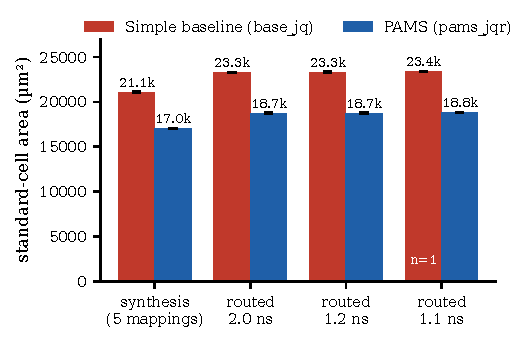
\includegraphics[width=\columnwidth]{figures/results/fig_area.pdf}
\caption{Standard-cell area: synthesis (median of 5 mappings) and routed cell area at three clock targets (median of valid seeds, error bars = min/max). At 1.1\ns{} only one baseline run is valid ($n = 1$).}\label{fig:area}
\end{figure}

\begin{figure}[t]\centering
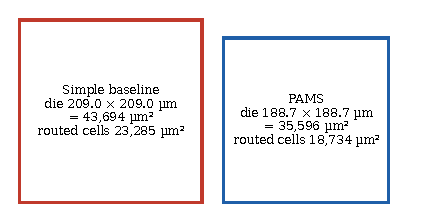
\includegraphics[width=\columnwidth]{figures/results/fig_die.pdf}
\caption{Estimated die footprint at 50\,\% utilization, drawn to scale (2.0\ns{} runs; the floorplan does not depend on the target).}\label{fig:die}
\end{figure}

\paragraph{Where the area goes.} \Cref{tab:resources} decomposes the synthesized area of mapping 0 by function (\file{paper/scripts/resources.py}; \cref{app:resources}). The 4,075\um{} difference comes from four sources:
\begin{itemize}
  \item 17 fewer gadgets: $17 \times 180.35 = 3{,}066\um$, three quarters of the saving;
  \item shorter delay chains: $-457\um$;
  \item the 14- instead of 24-bit share-wise operands without a mode shifter: $-1{,}286\um$ in front-end registers, logic and aligned operands;
  \item more public logic in \PAMS{}, which partly offsets the savings: $+873\um$ for $\Low_c$ and $\Theta_c$.
\end{itemize}

\begin{table}[t]\centering\small
\caption{Synthesized area by function (mapping 0, \si{\micro\meter\squared}). Combinational cells outside gadgets are attributed to the register group their fan-out reaches (approximate where ABC merged logic).}\label{tab:resources}
\setlength{\tabcolsep}{3pt}
\resizebox{\columnwidth}{!}{%
\begin{tabular}{@{}lrrr@{}}
\toprule
block & \PAMS{} & baseline & $\Delta$ \\
\midrule
HPC2 gadgets (40 / 57 $\times$ 180.35) & 7,214 & 10,280 & $-3{,}066$ \\
alignment (delay-chain) registers + logic & 3,558 & 4,016 & $-457$ \\
front-end registers ($x_r$, partial products, switched) & 1,081 & 1,411 & $-330$ \\
front-end logic (multipliers, sum, mode shift) & 2,610 & 3,033 & $-423$ \\
aligned operands $y_i$: registers + logic & 294 & 827 & $-533$ \\
public constant registers + logic & 1,337 & 464 & $+873$ \\
share-local XOR network at gadget inputs & 256 & 266 & $-10$ \\
input, control, accumulator, other & 672 & 801 & $-129$ \\
\midrule
total (equals reported synthesis area) & 17,022 & 21,097 & $-4{,}075$ \\
\bottomrule
\end{tabular}}
\end{table}

\subsection{Protected gadgets and randomness}
\Cref{fig:gadgets,fig:random} show the structural savings. The kernel needs 38 instead of 55 gadgets.
\begin{itemize}
  \item \textbf{CSA.} The narrower operands remove 10 of its gadgets.
  \item \textbf{Comparator.} The comparator against $\Theta_c$ on the low 11 bits plus the zero test of $Z_{13:11}$ (14 gadgets) replaces the baseline's carry-free zero test of its top 11 bits with an OR tree (20 gadgets). The ripple has two fewer carries.
  \item \textbf{Randomness.} Fresh randomness falls from 171 to 120 bits per cycle. At one coefficient per cycle, a generator must deliver \num{51} fewer bits every cycle. With 64-bit unrolled-Trivium instances~\cite{cassiers2024rng} that is two instances instead of three, but the generator is not included in any area figure.
\end{itemize}

\begin{figure}[t]\centering
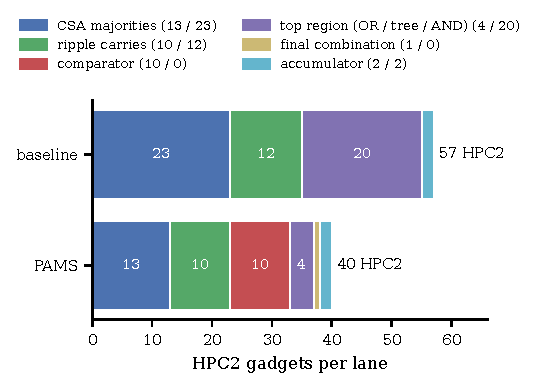
\includegraphics[width=\columnwidth]{figures/results/fig_gadgets.pdf}
\caption{HPC2 gadgets per lane by function (legend: \PAMS{} / baseline counts).}\label{fig:gadgets}
\end{figure}

\begin{figure}[t]\centering
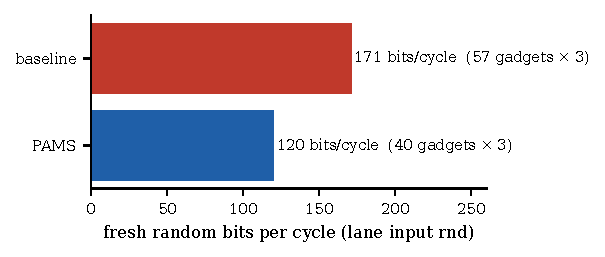
\includegraphics[width=\columnwidth]{figures/results/fig_random.pdf}
\caption{Fresh random bits consumed per cycle (3 per HPC2 gadget, second order).}\label{fig:random}
\end{figure}

\subsection{Timing}
\Cref{fig:timing} shows every run's achieved period.
\begin{itemize}
  \item \emph{2.0\ns{} target.} With no timing pressure, \PAMS{}'s median is 3.6\,\% lower. The baseline spreads widely across seeds (1.142--1.255\ns), and its fastest run beats PAMS's median. The distributions overlap ($p = 0.073$): \textbf{inconclusive}.
  \item \emph{1.2\ns{} target.} Timing-driven repair pulls both designs close to their limits, and the spread collapses to under 10\,ps. \PAMS{}'s period is lower in every seed ($p = 0.0006$), but only by 11\,ps (1.0\,\%). The seeds vary the layout of one netlist per design, so this separates the two layout distributions in this flow. It is not evidence of a general speed advantage (\cref{sec:method}).
  \item \emph{1.1\ns{} target.} \PAMS{} achieves 1.062--1.070\ns{} in all seven seeds. The only valid baseline run achieves 1.066\ns. Its five finished but DRC-failing runs reach 1.066--1.073\ns{}, so they show the same timing.
\end{itemize}
The two architectures have \textbf{comparable clock periods}. A difference of 1--4\,\% is not a timing advantage of practical size, and at the tightest target it disappears. \Cref{fig:adp} places every run in the area--delay plane: \PAMS{} occupies a lower band at every target, and its area-delay product is 19--23\,\% lower.

\begin{figure*}[t]\centering
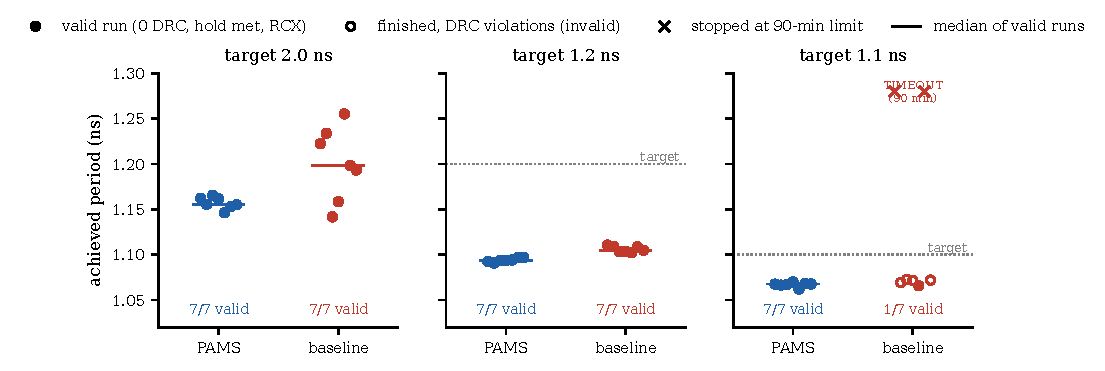
\includegraphics[width=\textwidth]{figures/results/fig_timing.pdf}
\caption{Achieved clock period of every P\&R run (seeds 1--7, offset horizontally by seed), at three targets. Filled = valid; hollow = finished with DRC violations; $\times$ = stopped at the 90-minute limit (no timing result).}\label{fig:timing}
\end{figure*}

\begin{figure}[t]\centering
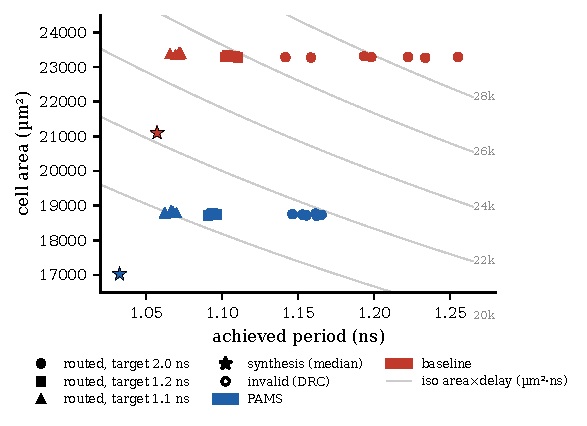
\includegraphics[width=\columnwidth]{figures/results/fig_adp.pdf}
\caption{Area versus achieved period for every routed run and for synthesis. Grey curves are iso-lines of area $\times$ delay.}\label{fig:adp}
\end{figure}

\paragraph{Why timing converges.} \Cref{fig:critpath} shows the worst routed paths at 1.2\ns.
\begin{itemize}
  \item \textbf{Both critical paths are in the share-wise front end.} \PAMS{} launches from \sig{x1r[5]} and captures at \sig{ml1[23]}: a partial product of the split constant multiplier, 1.057\ns{} of data path plus 0.179\ns{} of clock latency. The baseline's path, \sig{x0r[9]}$\to$\sig{mh0[31]}, has the same structure and a 1.073\ns{} data path.
  \item \textbf{Neither is in the masked kernel.} No gadget or comparator path is critical. Both front ends have been split until their stages balance near 1.0\ns{} (\cref{sec:method}).
  \item \textbf{The limit depends on the target.} Across all runs (\cref{tab:pnr-runs}), the limiting front-end stage changes:
  \begin{itemize}
    \item at 2.0\ns{}, \PAMS{} is limited by its public window logic (\sig{e0r}$\to$\sig{lowrq}), and the baseline by its mode-shift and offset stage (\sig{shp}$\to$\sig{y0}) or a partial product;
    \item at 1.2\ns{}, mostly by the partial products in both designs;
    \item at 1.1\ns{}, \PAMS{} by its public logic (\sig{c0r}$\to$\sig{lowrq}) and the baseline by its partial-product sum (\sig{mh}$\to$\sig{fq}).
  \end{itemize}
  \item \textbf{What remains.} The remaining difference is a few percent, between a 24-bit and a 34-bit constant multiplier stage and \PAMS{}'s public window stage. Further pipelining of either design, which for \PAMS{}'s public logic has no security cost, would reduce both periods toward a common limit set by the kernel. So we report no speed advantage.
\end{itemize}

\begin{figure*}[t]\centering
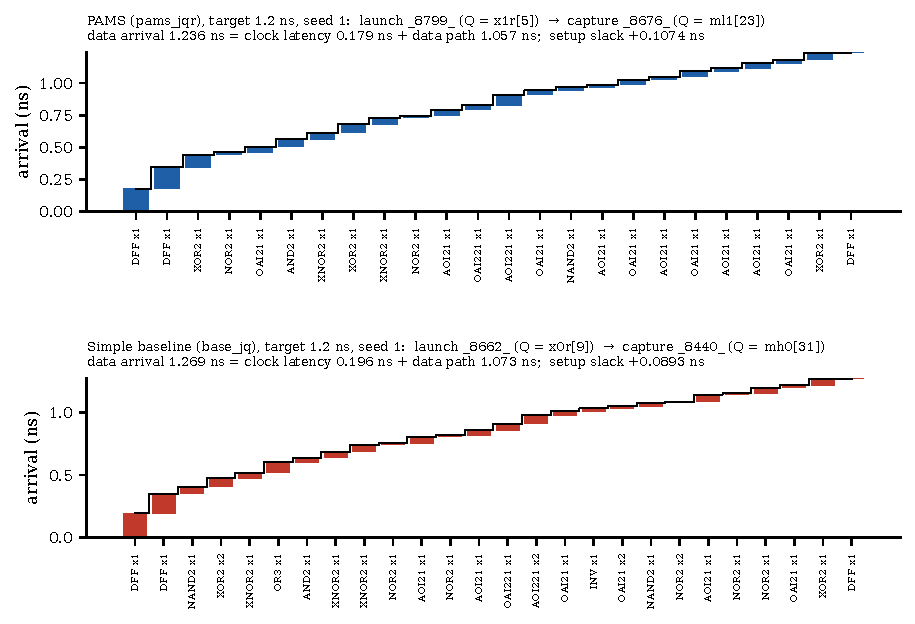
\includegraphics[width=\textwidth]{figures/physical/fig_critpath.pdf}
\caption{Worst setup paths of the routed reference runs (target 1.2\ns, seed 1), from OpenROAD \file{timing.rpt} on RCX parasitics. Bars = delay contributed by each cell (the first bar is the clock network latency at the launch flip-flop); black line = cumulative arrival. Both paths are a partial-product stage of the share-wise constant multiplier.}\label{fig:critpath}
\end{figure*}

\subsection{Physical realization and routability}
\Cref{fig:placement} (\cref{sec:circuit}) shows the placed designs at equal scale.
\begin{itemize}
  \item \textbf{Similar layouts.} In both designs the multipliers cluster near the input pins on the left, and the gadgets and delay chains fill the rest of the core.
  \item \textbf{Smaller PAMS core.} The \PAMS{} core is smaller in proportion to its cell area.
  \item \textbf{Less routing.} Total routed wirelength is \num{58067}--\num{58506}\,\si{\micro\meter} for \PAMS{} against \num{72529}--\num{73494}\,\si{\micro\meter} for the baseline at 1.1\ns, 20\,\% less.
\end{itemize}

At the 1.1\ns{} target this difference matters for routing (\cref{fig:routing}):
\begin{itemize}
  \item \textbf{PAMS:} every run routed DRC-clean in about 1.3 minutes.
  \item \textbf{Baseline:} only seed 5 did. Four runs finished with 1--6 residual DRC violations after 64 detailed-routing iterations (31--63 minutes), and two exceeded the 90-minute limit.
\end{itemize}

This is a flow-specific observation at one utilization: a lower utilization would probably let the baseline route, at a larger die. It shows that the smaller \PAMS{} netlist is easier to route under timing pressure in this flow, not that \PAMS{} is generally more routable. One valid baseline run is a single sample, not a distribution.

\begin{figure}[t]\centering
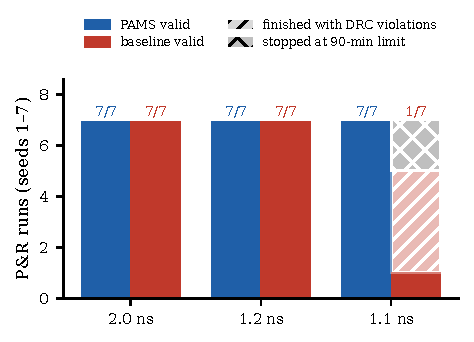
\includegraphics[width=\columnwidth]{figures/results/fig_routing.pdf}
\caption{Routing outcome of the seven seeds per design and target. At 1.1\ns, the baseline finished DRC-clean once, finished with DRC violations four times and was stopped twice.}\label{fig:routing}
\end{figure}

\subsection{Comparison with the original baseline}
Our first study compared the original, unpipelined designs. It reported \num{21.3}\,\% less area and \num{10.4}\,\% lower routed clock period against that original baseline. The area figure largely survives against the optimized baseline. The delay figure does not: it came from the original baseline's unpipelined 34-bit multiplier, and it vanishes once both designs are pipelined equally. We report it only as a historical comparison against a weaker baseline.
